\subsection{Correlation method}
a simple absolute correlation can be applied to the list of genes. The adjustable parameters are:

\begin{itemize}
\item Correlation type (Pearson, Spearman, Kendall)
\item Correlation coefficient
\item Correlation p-value
\end{itemize}

Optionally, a linear model fit can be overlayed on the scatterplot graph.

\begin{center}
	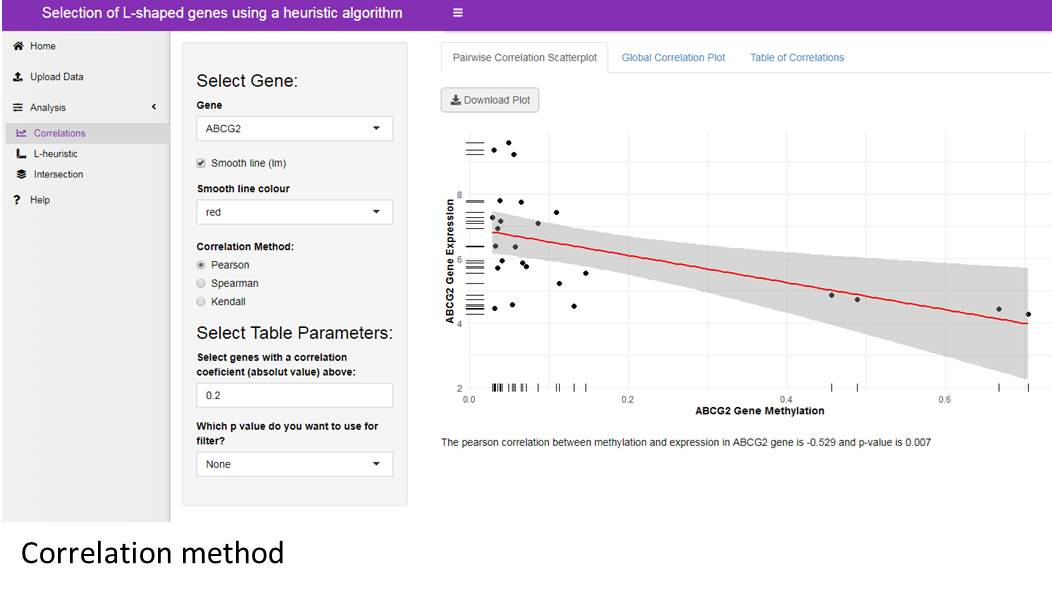
\includegraphics[width=0.8\columnwidth]{./images/correlation_method.png}
\end{center}

